% Decoder-side serving loop for the causal streaming backend: what one
% ~2 s update actually forwards. Same visual language as offline_vs_causal.tex.
% Compile: lualatex causal_streaming.tex ; export: pdftocairo -svg
\documentclass[tikz,border=10pt]{standalone}
\usepackage{amssymb}
\usetikzlibrary{arrows.meta,calc,decorations.pathreplacing,positioning}
\renewcommand{\familydefault}{\sfdefault}

\definecolor{boxgray}{HTML}{D9D9D9}
\definecolor{boxedge}{HTML}{8A8A8A}
\definecolor{tokteal}{HTML}{7FD6C2}
\definecolor{toktealmute}{HTML}{C8EDE4}
\definecolor{toklilac}{HTML}{E7E1F7}
\definecolor{labelpurple}{HTML}{6C4FD8}
\definecolor{inkgray}{HTML}{5A5A5A}
\definecolor{accent}{HTML}{0A66A3}
\definecolor{accentlight}{HTML}{D7E7F3}
\definecolor{okgreen}{HTML}{6B9E3F}
\definecolor{warm}{HTML}{C2542E}
\definecolor{mute}{HTML}{C9C9C9}

\begin{document}
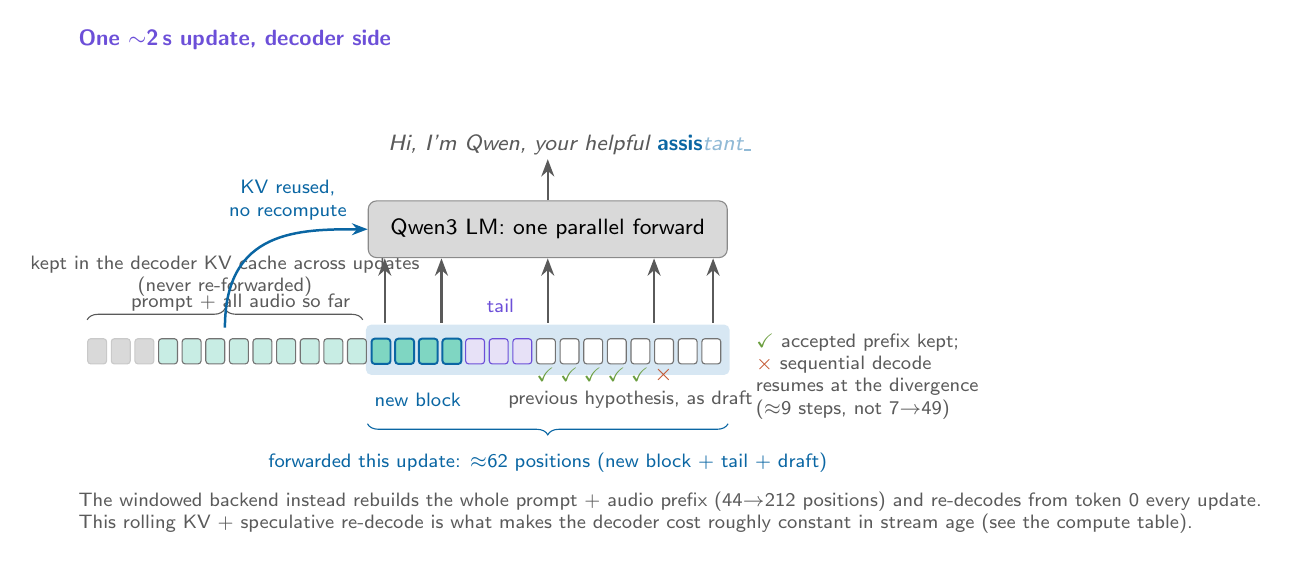
\begin{tikzpicture}[
  font=\footnotesize,
  bigbox/.style={rounded corners=3pt, draw=boxedge, fill=boxgray,
                 minimum height=0.72cm, inner xsep=8pt},
  tok/.style={rounded corners=1.1pt, minimum width=0.24cm, minimum height=0.32cm,
              inner sep=0, draw=black!55, line width=0.4pt, anchor=west},
  glbl/.style={inkgray, font=\scriptsize, inner sep=1pt},
  plbl/.style={labelpurple, font=\footnotesize\itshape, inner sep=1pt},
  flow/.style={-{Stealth[length=2.2mm]}, inkgray, line width=0.9pt},
]

\def\step{0.30}
% group start x and counts
% head 0.0 (3) | cachedA 0.9 (9) | newblk 3.6 (4) | tail 4.8 (3) | draft 5.7 (8)

\node[plbl, anchor=west] at (-0.15, 3.95) {\textbf{One $\sim$2\,s update, decoder side}};

% ---- forwarded-region highlight behind new block + tail + draft ----
\fill[accentlight, rounded corners=2pt] (3.54, -0.30) rectangle (8.16, 0.34);

% ---- token strip ----
\foreach \i in {0,...,2}{ \node[tok, fill=boxgray, draw=mute] at (0.0+\i*\step, 0) {}; }
\foreach \i in {0,...,8}{ \node[tok, fill=toktealmute] at (0.9+\i*\step, 0) {}; }
\foreach \i in {0,...,3}{ \node[tok, fill=tokteal, draw=accent, line width=0.7pt] at (3.6+\i*\step, 0) {}; }
\foreach \i in {0,...,2}{ \node[tok, fill=toklilac, draw=labelpurple] at (4.8+\i*\step, 0) {}; }
\foreach \i in {0,...,7}{ \node[tok, fill=white] at (5.7+\i*\step, 0) {}; }

% ---- group labels above strip ----
\node[glbl, align=center] at (1.95, 0.62) {prompt + all audio so far};
\node[glbl, accent, align=center] at (4.2, -0.62) {new block};
\node[glbl, labelpurple, align=center] at (5.25, 0.58) {tail};
\node[glbl, align=center] at (6.9, -0.62) {previous hypothesis, as draft};

% ---- kept-in-KV brace (head + cached audio) ----
\draw[decorate, decoration={brace, amplitude=4pt}, inkgray]
  (0.0, 0.40) -- (3.50, 0.40);
\node[glbl, align=center] at (1.75, 0.95) {kept in the decoder KV cache across updates\\(never re-forwarded)};

% ---- forwarded-region brace ----
\draw[decorate, decoration={brace, mirror, amplitude=4pt}, accent]
  (3.56, -0.92) -- (8.14, -0.92);
\node[glbl, accent, align=center] at (5.85, -1.42)
  {forwarded this update: $\approx$62 positions (new block + tail + draft)};

% ---- verification marks under the draft ----
\foreach \i in {0,...,4}{ \node[okgreen, font=\scriptsize] at (5.82+\i*\step, -0.30) {\checkmark}; }
\node[warm, font=\footnotesize\bfseries] at (5.82+5*\step, -0.30) {$\times$};

% ---- LM box over the forwarded region ----
\node[bigbox, minimum width=4.55cm] (lm) at (5.85, 1.55) {Qwen3 LM: one parallel forward};
\foreach \x in {3.78, 4.5, 5.85, 7.2, 7.95}{ \draw[flow] (\x, 0.36) -- (\x, 1.18); }

% ---- KV-reuse arrow from kept region into the LM box ----
\draw[-{Stealth[length=2mm]}, accent, line width=0.9pt]
  (1.75, 0.30) .. controls (1.75, 1.55) and (2.7, 1.55) .. (lm.west);
\node[glbl, accent, align=center] at (2.55, 1.92) {KV reused,\\no recompute};

% ---- accepted vs resume annotation ----
\node[glbl, align=left, anchor=west] at (8.45, -0.32)
  {\textcolor{okgreen}{\checkmark} accepted prefix kept;\\\textcolor{warm}{$\times$} sequential decode\\resumes at the divergence\\($\approx$9 steps, not 7$\to$49)};

% ---- output text (committed / fresh / faded), figure-1 convention ----
\node[anchor=west, font=\footnotesize\itshape] at (3.7, 2.62)
  {\textcolor{inkgray}{Hi, I'm Qwen, your helpful}\ \textcolor{accent}{\textbf{assis}}\textcolor{accent!45}{tant\_}};
\draw[flow] (5.85, 1.92) -- (5.85, 2.44);

% ---- caption ----
\node[glbl, anchor=west, align=left] at (-0.15, -2.05)
  {The windowed backend instead rebuilds the whole prompt + audio prefix (44$\to$212 positions) and re-decodes from token 0 every update.\\This rolling KV + speculative re-decode is what makes the decoder cost roughly constant in stream age (see the compute table).};

\end{tikzpicture}
\end{document}
